% Created 2018-04-02 lun 17:36
% Intended LaTeX compiler: pdflatex
\documentclass[xcolor={usenames,svgnames,dvipsnames}]{beamer}
\usepackage[utf8]{inputenc}
\usepackage[T1]{fontenc}
\usepackage{graphicx}
\usepackage{grffile}
\usepackage{longtable}
\usepackage{wrapfig}
\usepackage{rotating}
\usepackage[normalem]{ulem}
\usepackage{amsmath}
\usepackage{textcomp}
\usepackage{amssymb}
\usepackage{capt-of}
\usepackage{hyperref}
\usepackage{color}
\usepackage{listings}
\usepackage{mathpazo}
\usepackage{gensymb}
\usepackage{amsmath}
\usepackage{chemarr}%flechas para reacciones químicas (SFER.tex)
\bibliographystyle{plain}
\AtBeginSubsection[]{\begin{frame}[plain]\tableofcontents[currentsubsection,sectionstyle=show/shaded,subsectionstyle=show/shaded/hide]\end{frame}}
\AtBeginSection[]{\begin{frame}[plain]\tableofcontents[currentsection,hideallsubsections]\end{frame}}
\usepackage[emulate=units]{siunitx}
\sisetup{fraction=nice, decimalsymbol=comma, retain-unity-mantissa = false}
\newunit{\wattpeak}{Wp}
\newunit{\watthour}{Wh}
\newunit{\amperehour}{Ah}
\hypersetup{colorlinks=true, linkcolor=Blue, urlcolor=Blue}
\renewcommand{\thefootnote}{\fnsymbol{footnote}}
\setbeamercolor{alerted text}{fg=blue!50!black} \setbeamerfont{alerted text}{series=\bfseries}
\usetheme[hideothersubsections]{Goettingen}
\usecolortheme{rose}
\usefonttheme{serif}
\author{Oscar Perpiñán Lamigueiro \\ \url{http://oscarperpinan.github.io}}
\date{}
\title{Solar Radiation on a Horizontal Plane}
\subtitle{Fundamentals of PV Engineering}
\hypersetup{
 pdfauthor={Oscar Perpiñán Lamigueiro \\ \url{http://oscarperpinan.github.io}},
 pdftitle={Solar Radiation on a Horizontal Plane},
 pdfkeywords={},
 pdfsubject={},
 pdfcreator={Emacs 25.2.2 (Org mode 9.1.9)}, 
 pdflang={Spanish}}
\begin{document}

\maketitle

\section{Motivation}
\label{sec:org8336c0c}
\begin{frame}[label={sec:org70f65bf}]{Solar Variability}
\begin{itemize}
\item Extraterrestrial solar radiation is a deterministic process (it depends on latitude, day of year, and time of day).
\item However, global radiation is a stochastic (random) process because of the interaction with the atmosphere:
\begin{itemize}
\item Time variability
\item Spatial variability
\end{itemize}
\end{itemize}
\end{frame}
\begin{frame}[label={sec:org8ddb3cd}]{Long-term Estimations}
\begin{itemize}
\item We are interested in \alert{long-term estimations} of the performance of PV systems in a definite location.
\item Solar radiation data sources must \alert{capture the long-term behaviour} (interannual variability) and be \alert{representative of the specified location} (spatial variability).
\end{itemize}
\end{frame}

\begin{frame}[label={sec:org2c2d0db}]{Time Variability}
\begin{center}
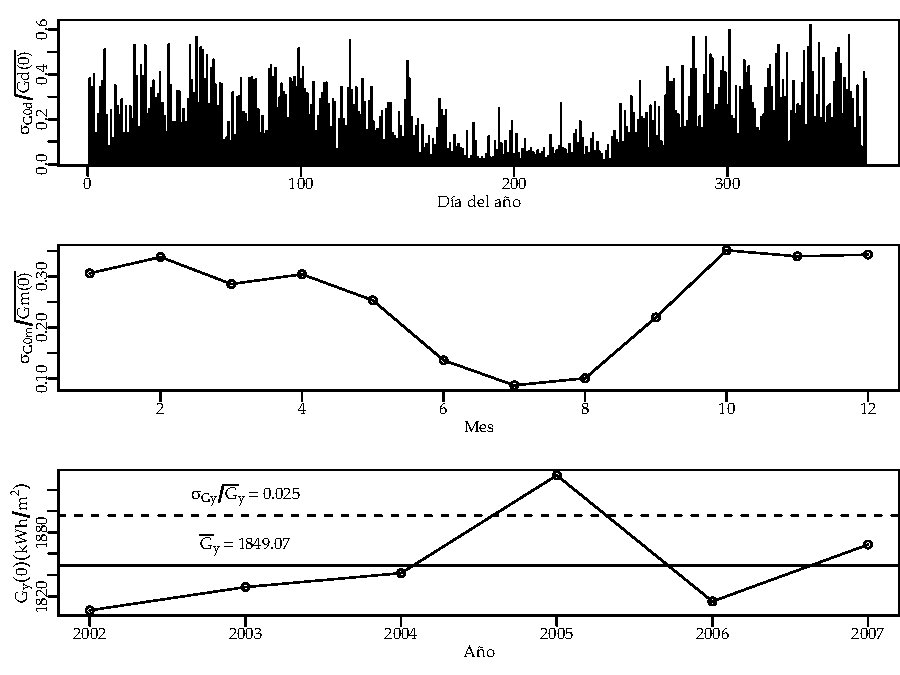
\includegraphics[height=0.4\textheight]{../figs/VariabilidadRadiacionDiario.pdf}
\end{center}

\begin{block}{Key concepts}
\begin{itemize}
\item Time variability \alert{increases with time resolution} (higher for daily values than for monthly averages).
\item Fluctuations are \alert{higher in winter than in summer}.
\item Reproducing \alert{long-term trends} requires \alert{long time series} (about 10 years length).
\end{itemize}
\end{block}
\end{frame}

\begin{frame}[label={sec:orgeb6f713}]{Spatial Variability}
\begin{center}
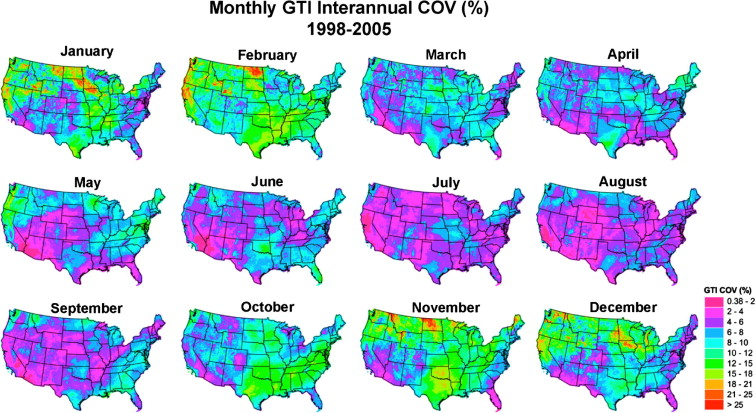
\includegraphics[height=0.4\textheight]{../figs/SpatialVariability.jpg}
\end{center}

\begin{block}{Key concepts}
\begin{itemize}
\item Spatial variability depends on the \alert{local climatology}.
\item Spatial variability is \alert{higher in winter than in summer} (for a same location).
\item Measurements are representative of nearby locations for a \alert{limited distance} (about 10 kms.)
\end{itemize}
\end{block}
\end{frame}

\begin{frame}[label={sec:orgb179055}]{Summary: Measurements requirements}
\begin{itemize}
\item Reliable and representative long-term estimations of PV performance require:
\begin{itemize}
\item \alert{Nearby measurements}: \(\leq \SI{10}{km}\)
\item \alert{Long time series}: \(\simeq \SI{10}{years}\)
\end{itemize}
\end{itemize}
\end{frame}

\section{Data Sources}
\label{sec:org3f7af16}
\begin{frame}[label={sec:org2a628ea}]{Meteorological stations}
\begin{itemize}
\item Long time series.
\item High time resolution (\(\SI{1}{\min}\))
\item Low spatial resolution (point measurements).
\item Errors due to meter inaccuracy (no models required).
\end{itemize}

\begin{block}{Pyranometer}
\end{block}
\begin{columns}
\begin{column}{0.4\columnwidth}
\begin{center}
\begin{center}
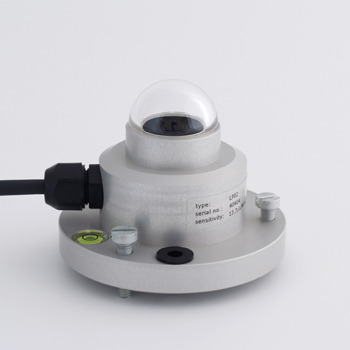
\includegraphics[width=0.8\textwidth]{../figs/piranometro.jpg}
\end{center}
\end{center}
\end{column}
\end{columns}
\end{frame}


\begin{frame}[label={sec:org81dcadf}]{Satellite imaging}
\begin{itemize}
\item Low time resolution (\(\SI{1}{hour}\) or \(\SI{1}{day}\)).

\item High spatial resolution (\(\SI{15}{km}\)).

\item Global solar radiation is estimated by processing images of the satellite radiometers.

\item Errors due model inaccuracy (radiation is estimated).
\end{itemize}
\end{frame}


\begin{frame}[label={sec:orgdb620e9}]{Hybrid methods}
\begin{itemize}
\item Ground measurements merged with satellite estimations to increase spatial resolution.
\item Spatial interpolation
\begin{itemize}
\item \alert{Inverse Distance Weighting (IDW)} (\(d\) is the distance between locations \(x_0\) and \(x_i\))
\[
\widehat{G}_d(x_0) = \frac{\sum_{i=1}^N w_i G_{d}(x_i)}{\sum_{i=1}^N w_i} 
\]

\[
  w_i = 1/d^2(x_0, x_i)
\]
\item \alert{Ordinary Kriging}
\item \alert{Kriging with External Drift (KED)}
\end{itemize}
\end{itemize}
\end{frame}

\begin{frame}[label={sec:orgb226503}]{Data sources}
\begin{block}{Wiki}
\url{https://github.com/oscarperpinan/mds/wiki}
\end{block}
\end{frame}

\begin{frame}[label={sec:org5c1718d}]{Data sources}
\begin{block}{Meteorological Stations}
\url{https://github.com/oscarperpinan/mds/wiki/stations}
\end{block}
\end{frame}

\begin{frame}[label={sec:org93845ec}]{Data sources}
\begin{block}{Satellite Estimations}
\begin{itemize}
\item NASA: \url{https://github.com/oscarperpinan/mds/wiki/nasa}
\item CM SAF: \url{https://github.com/oscarperpinan/mds/wiki/cmsaf}
\item LSA SAF: \url{https://github.com/oscarperpinan/mds/wiki/lsasaf}
\end{itemize}
\end{block}
\end{frame}

\begin{frame}[label={sec:org5fe8ae1}]{Data sources}
\begin{block}{Hybrid estimations}
\begin{itemize}
\item PVGIS: \url{https://github.com/oscarperpinan/mds/wiki/pvgis}
\item ADRASE: \url{https://github.com/oscarperpinan/mds/wiki/adrase}
\end{itemize}
\end{block}
\end{frame}

\section{Quality Control}
\label{sec:orgb669fde}
\begin{frame}[label={sec:org20e3531}]{Motivation}
\begin{itemize}
\item Measurements must be filtered and corrected to remove erroneous data and outliers.
\begin{itemize}
\item Physical limits
\item Spatial coherence
\item Statistical analysis of deviations
\end{itemize}
\end{itemize}
\end{frame}


\begin{frame}[label={sec:org84eb724}]{Physical limits}
\begin{itemize}
\item Daily clearness index\footnote{Clearness index is defined as the ratio \(K_{dT} = G_d(0) / B_{0d}(0)\).} cannot exceed 1 (daily global irradiation cannot exceed extraterrestrial solar irradiation).
\end{itemize}
\[
  K_{dT} \leq 1
\]

\[
G_d(0) \leq B_{0d}(0)
\]

\begin{itemize}
\item Clearness index must be higher than 0.03
\end{itemize}
\[
K_t = \frac{G_d(0)}{B_{0d}(0)} \geq 0.03
\]
\end{frame}

\begin{frame}[label={sec:orgf5bd61e}]{Spatial coherence}
\begin{itemize}
\item Measurements from a station should be compared with \alert{nearby stations} (for example, using spatial interpolation)
\item Comparison must be established with \alert{aggregated values} (daily or monthly averages).
\end{itemize}
\end{frame}

\begin{frame}[label={sec:org225bce2}]{Statistical Analysis of Deviations}
\begin{itemize}
\item Statistical analysis of the deviations, \(\mathbf{D}\), between Observations, \(\mathbf{O}\), and a Model, \(\mathbf{M}\) (or another set of observations):
\end{itemize}

\[
\mathbf{O} = \left\{ o_1 \dots o_n \right\}
\]

\[
\mathbf{M} = \left\{ m_1 \dots m_n  \right\}
\]

\[
\mathbf{D} = \mathbf{M} - \mathbf{O} =  \left\{ (m_1 - o_1) \dots (m_n - o_n)  \right\} = \left\{ d_1 \dots d_n  \right\}
\]
\end{frame}

\begin{frame}[label={sec:orga3f804c}]{Metrics}
\begin{itemize}
\item Mean Bias Difference (MBD):
\end{itemize}
\[
MBE = \overline{\mathbf{D}} = \overline{\mathbf{M}} - \overline{\mathbf{O}} = \frac{1}{n} \sum_{i=1}^n (m_i - o_i)
\]

\begin{itemize}
\item Root Mean Square Error (RMSD):
\end{itemize}
\[
RMSD = \left(\frac{1}{n} \sum_{i=1}^n d_i^2 \right)^{1/2} =  \left( \frac{1}{n} \sum_{i=1}^n (m_i - o_i)^2  \right)^{1/2}
\]

\begin{itemize}
\item Mean Absolute Deviation (MAD):
\end{itemize}

\[
MAD = \frac{1}{n} \sum_{i=1}^n \left|d_i\right| =  \frac{1}{n} \sum_{i=1}^n \left|m_i - o_i\right|
\]
\end{frame}
\end{document}